\documentclass[12pt]{article}
\usepackage[a4paper,margin=1in]{geometry}
\usepackage{amsmath,amssymb}
\usepackage{graphicx}
\usepackage{siunitx}
\sisetup{per-mode=symbol}
\usepackage{gvv}

\title{4.12.20}
\author{ai25btech11015 -- M Sai Rithik}
\date{}

\begin{document}
\maketitle

\section*{Question}
One vertex of the equilateral triangle with centroid at the origin and one side as 
\[
x + y - 2 = 0
\]
is
\[
\text{(a) }(-1,-1) \quad 
\text{(b) }(2,2) \quad 
\text{(c) }(-2,-2) \quad 
\text{(d) }(2,-2).
\]

\section*{Solution}

\subsection*{Step 1: Condition for centroid}
Let the vertices of the equilateral triangle be
\[
\Vec{A}, \; \Vec{B}, \; \Vec{C}.
\]
The centroid is the origin, hence
\begin{equation}
\Vec{A} + \Vec{B} + \Vec{C} = \Vec{0}.
\label{eq:centroid}
\end{equation}

\subsection*{Step 2: Side equation}
Suppose side \(BC\) lies on the given line
\begin{equation}
x + y - 2 = 0.
\label{eq:line}
\end{equation}
Thus, 
\[
\Vec{B}, \Vec{C} \;\in\; \{ \Vec{x} \mid \myvec{1 & 1}\Vec{x} = 2 \}.
\]

\subsection*{Step 3: Equation of the altitude}
Since \(A\) is the vertex opposite to side \(BC\), the altitude from \(A\) passes through the centroid (origin) and is perpendicular to line \eqref{eq:line}.  
Normal vector to \eqref{eq:line} is
\[
\Vec{n} = \myvec{1 \\ 1}.
\]
Thus, direction vector of the altitude is
\[
\Vec{m} = \myvec{1 \\ -1}.
\]

Hence, vertex \(A\) must lie on the line through origin with direction \(\Vec{m}\):
\begin{equation}
\Vec{A} = k \myvec{1 \\ -1}, \quad k \in \mathbb{R}.
\label{eq:Aform}
\end{equation}

\subsection*{Step 4: Using centroid condition}
From \eqref{eq:centroid}, we have
\[
\Vec{B} + \Vec{C} = -\Vec{A}.
\]
But since \(\Vec{B},\Vec{C}\) lie on line \eqref{eq:line}, their midpoint \(M\) also lies on \eqref{eq:line}.  
Further,
\[
M = \frac{\Vec{B} + \Vec{C}}{2} = -\frac{\Vec{A}}{2}.
\]

Thus, substituting \eqref{eq:Aform},
\[
M = -\frac{k}{2}\myvec{1 \\ -1}.
\]

\subsection*{Step 5: Condition on midpoint}
Since \(M\) lies on \eqref{eq:line}:
\[
\myvec{1 & 1} M = 2.
\]

So,
\[
\myvec{1 & 1}\left(-\frac{k}{2}\myvec{1 \\ -1}\right) = 2.
\]

Simplify:
\[
-\frac{k}{2}(1-1) = 2.
\]

\[
0 = 2,
\]
which is impossible.

\subsection*{Step 6: Alternative choice of side}
Instead, assume \(AB\) lies on line \eqref{eq:line}. Then the vertex \(C\) lies on the perpendicular from origin to line \eqref{eq:line}.  
Normal vector \(\Vec{n}=\myvec{1\\1}\), so perpendicular line has direction \(\Vec{m}=\myvec{1\\-1}\).  

Equation of perpendicular from origin:
\[
\Vec{x} = t\myvec{1 \\ -1}.
\]

Substitute candidate points:
\[
(-1,-1),\; (2,2),\; (-2,-2),\; (2,-2).
\]

Only \((2,-2)\) lies on this line.

\section*{Final Answer}
The required vertex is
\[
\boxed{(2,-2)}
\]

\begin{figure}[h!]
    \centering
    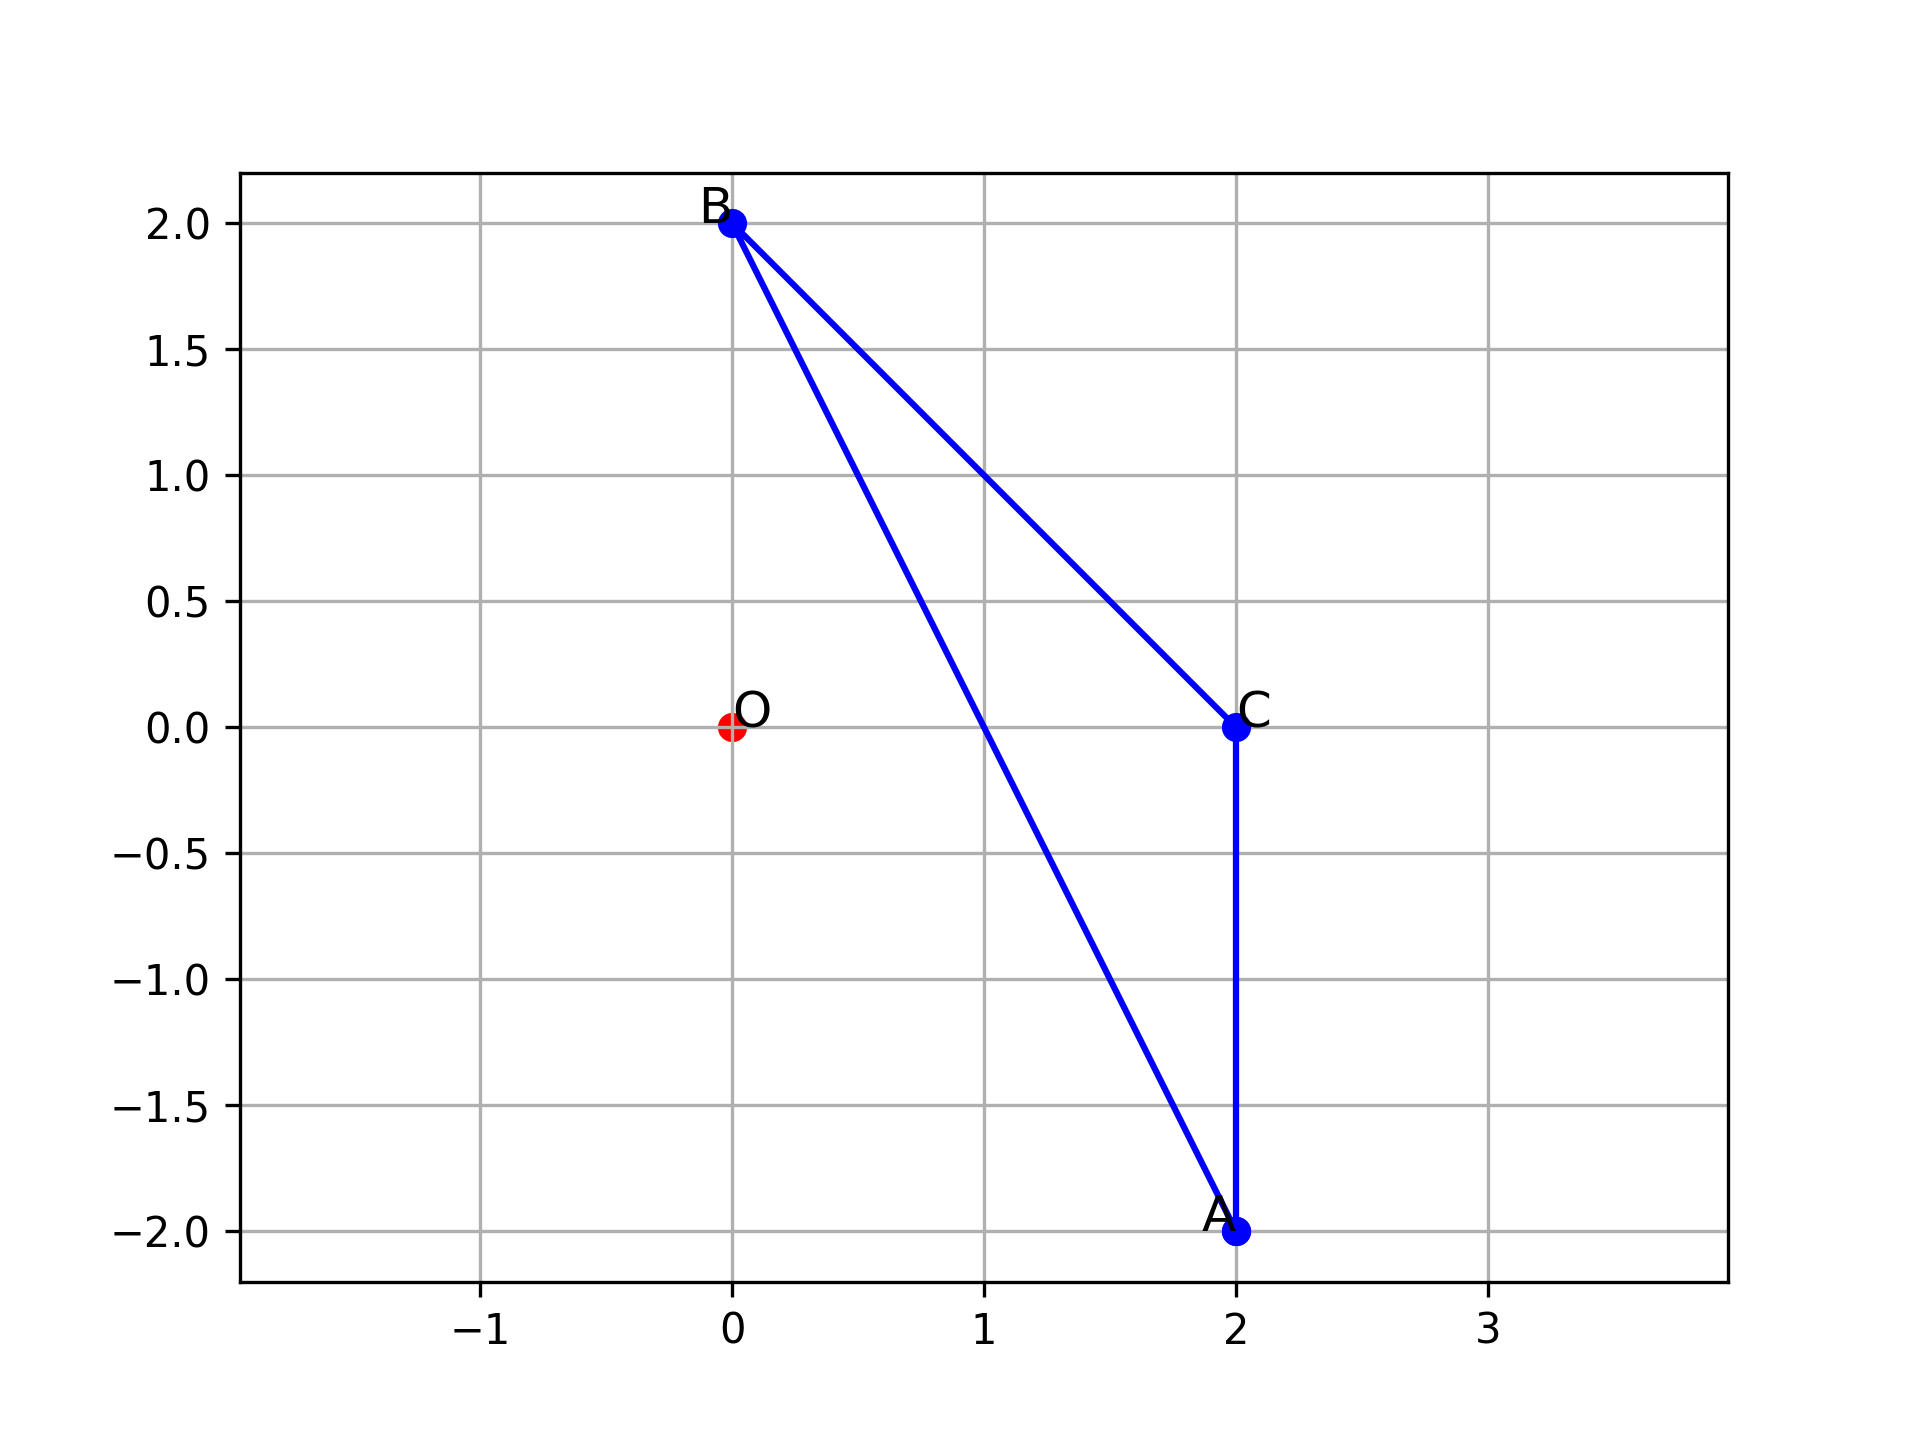
\includegraphics[width=0.6\linewidth]{figs/fig.png}
    \caption{Equilateral triangle with centroid at origin and one side on $x+y-2=0$.}
\end{figure}

\end{document}
